% Straight up stealing preamble from Eli Holmes 
%%%%%%%%%%%%%%%%%%%%%%%%%%%%%%%%%%%%%%START PREAMBLE THAT IS THE SAME FOR ALL EXAMPLES
\documentclass{article}

%Required: You must have these


\usepackage{authblk}
\documentclass{article}
\usepackage{Sweave}
\usepackage{graphicx}
\usepackage{tabularx}
\usepackage{hyperref}
\usepackage{natbib}
\usepackage{pdflscape}
\usepackage{array}
\usepackage{gensymb}
\usepackage{amsmath}
\usepackage{longtable}
\usepackage{xr}
\usepackage[small]{caption}
\renewcommand{\baselinestretch}{1.8}
%\usepackage{lineno}
%\usepackage[backend=bibtex]{biblatex}
%Strongly recommended
 %put your figures in one place
 
%you'll want these for pretty captioning
\usepackage[small]{caption}

\setkeys{Gin}{width=0.8\textwidth} %make the figs 50 perc textwidth
\setlength{\captionmargin}{30pt}
\setlength{\abovecaptionskip}{0pt}
\setlength{\belowcaptionskip}{10pt}
% manual for caption http://www.dd.chalmers.se/latex/Docs/PDF/caption.pdf

%Optional: I like to muck with my margins and spacing in ways that LaTeX frowns on
%Here's how to do that
 \topmargin -2cm 
 \oddsidemargin -0.04cm 
 \evensidemargin -0.04cm % same as oddsidemargin but for left-hand pages
 \textwidth 16.59cm
 \textheight 22.94cm 
 %\pagestyle{empty} % Uncomment if don't want page numbers
 %\parskip 7.2pt  % sets spacing between paragraphs
 %\renewcommand{\baselinestretch}{1.5} 	% Uncomment for 1.5 spacing between lines
\parindent 0pt% sets leading space for paragraphs
\usepackage[doublespacing]{setspace}
%\doublespacing

%Optional: I like fancy headers
\usepackage{fancyhdr}
\pagestyle{fancy}
\fancyhead[LO]{Soil moisture and plant phenology}
\fancyhead[RO]{2018}

%%%%%%%%%%%%%%%%%%%%%%%%%%%%%%%%%%%%%%END PREAMBLE THAT IS THE SAME FOR ALL EXAMPLES

%Start of the document
\begin{document}

% \SweaveOpts{concordance=TRUE}
\bibliographystyle{amnat.bst}

\title{Supplemental Materials for \emph{Soil moisture interacts with temperature to affect plant phenology}}
\begin{singlespace}

\author[1,2,a]{A.K. Ettinger}
\author[3,b]{J.S. Dukes}
\author[4,c]{M.R. Johnston}
\author[5,d]{C.R. Rollinson}
\author[1,4,6,e]{E.M. Wolkovich}

\affil[1]{Arnold Arboretum of Harvard University, Boston, Massachusetts 02131, USA}

\affil[2]{The Nature Conservancy,74 Wall Street, Seattle, Washington, 98121}


\affil[3]{Department of Forestry \& Natural Resources and Department of Biological Sciences, Purdue University, West Lafayette, Indiana 47907, USA}

\affil[4]{Department of Organismic \& Evolutionary Biology, Harvard University, Cambridge, Massachusetts 02138, USA}

\affil[5]{The Morton Arboretum, Lisle, Illinois 60532, USA}

\affil[6]{Forest \& Conservation Sciences, Faculty of Forestry, University of British Columbia, Vancouver, BC, Canada}

\affil[a]{Corresponding author; email:ailene.ettinger@tnc.org; phone: 781-296-4821; mailing address: 74 Wall Street, Seattle, Washington, 98121 USA }

%\affil[d]{jsdukes@purdue.edu}

%\affil[f]{mjohnston@g.harvard.edu}

%\affil[h]{crollinson@mortonarb.org}

%\affil[j]{e.wolkovich@ubc.ca}

\date{\today}
\maketitle %put the fancy title on
%\tableofcontents %add a table of contents

%\textbf{Statement of authorship} 
%All authors conceived of this manuscript, which began at a Radcliffe Exploratory Seminar in 2016, and all authors contributed to manuscript revisions. AKE and EMW conceived of the idea for the literature review, database compilation, and related Radcliffe Exploratory Seminar. AKE compiled the datasets; AKE analyzed the data and created the figures; AKE wrote the manuscript.

%\textbf{Data Accessibility} %Data accessibility statement: The statement must confirm that, should the manuscript be accepted, the data supporting the results will be archived in an appropriate public repository such as Dryad or Figshare and the data DOI will be included at the end of the article.
%The MC3E and ExPhen databases are available at KNB \citep{ettinger2018}, along with all R code from the analyses included in this paper. (Currently, metadata are published there; the full databases and R code are available to reviewers on github.) 

%\textbf{Running title} 
%\textbf{Key words} global warming, warming experiment, microclimate, phenology, direct and indirect effects, active-warming, target temperature
\end{singlespace}


\clearpage
%%%%%%%%%%%%%%%%%%%%%%%%%%%%%%%%%%%%%%%%%%%%%%%%%%%
%\linenumbers

\section* {Supplemental Methods}
\underline{Equation for phenology models}: 
Response variable (\textit{y}) is day of year of the phenological event (budburst, leafout, or flowering). Predictors are measured air temperature (\textit{T}) and soil moisture(\textit{SM}). Random effects are species (sp, random slopes and intercepts), and  site and year nested within site (random intercepts).

%\begin{equation}
\begin{equation}
y_{i}=\alpha_{sp[i],site[year[i]]} + \beta_{temp_{sp[i]}}+ \beta_{mois_{sp[i]}} + \beta_{temp:mois_{sp[i]}}+\epsilon_{i}\label{eq:8}
\end{equation}

\begin{equation}
\alpha_{sp}\sim N(\mu_{sp}, \sigma_{sp})
\end{equation}

\begin{equation}
\mu_{site[year]} \sim N(\mu_{siteyr}, \sigma_{siteyr})
\end{equation}

\begin{equation}
\mu_{site} \sim N(\mu_{site}, \sigma_{site})
\end{equation}

\begin{equation}
\beta_{temp_{sp}} \sim N(\mu_{\beta_{temp}}, \sigma_{\beta_{temp}})
\end{equation}

\begin{equation}
\beta_{mois_{sp}} \sim N(\mu_{\beta_{mois}}, \sigma_{\beta_{mois}})
\end{equation}

\begin{equation}
\beta_{temp:mois_{sp}} \sim N(\mu_{\beta_{temp:mois}}, \sigma_{\beta_{temp:mois}})
\end{equation}


% \underline{Equations for soil moisture and temeprature models}: 
% The equations below represent the models we used to understand effects of experimental temperature (\textit{eT}) and experimental preciptation (\textit{eP}) treatments treatments on soil moisture and temperature. Since the model structures for our analyses of moisture and temperature were identical, \textit{y} represents either moisture or temperature. 
% 
% \begin{equation}
% y_{i}=\alpha_{site[year[doy[i]]]}+ \beta_{temp_{site[i]}}eT_i+\beta_{2 site[i]}eP_i+\beta_{3 site[i]}eT_ieP_i+\epsilon_{i}\label{eq:1}
% \end{equation}
% \begin{equation}
% \alpha_{site[year[doy]]}\sim N(\mu_{site[year]}, \sigma_{site[year]})\label{eq:2}
% \end{equation}
% 
% \begin{equation}
% \mu_{site[year]} \sim N(\mu_{sy}, \sigma_{sy})\label{eq:3}
% \end{equation}
% 
% \begin{equation}
% \mu_{sy} \sim N(\mu_{s}, \sigma_{s})\label{eq:4}
% \end{equation}
% 
% \begin{equation}
% \beta_{1 site} \sim N(\mu_{\beta1}, \sigma_{\beta1})\label{eq:5}
% \end{equation}
% 
% \begin{equation}
% \beta_{2 site} \sim N(\mu_{\beta2}, \sigma_{\beta2})\label{eq:6}
% \end{equation}
% 
% \begin{equation}
% \beta_{3 site} \sim N(\mu_{\beta3}, \sigma_{\beta3})\label{eq:7}
% \end{equation}
% 
% 
% 
% \section* {Results}
% \begin{singlespace}


\bibliography{../../Bibliography/mylibrary.bib}

\section*{References to include}
\begin{itemize}
\item Later flowering is  associated with low precipitation, at least in part (Crimmins et al 2010)
\item Ganjurjav et al 2020
\item Cabon 2020
\end{itemize}

\clearpage
\section* {Supplemental Tables}

% latex table generated in R 4.1.3 by xtable 1.8-4 package
% Fri Sep 23 17:05:34 2022
\begin{table}[ht]
\centering
\caption{\textbf{Experimental sites and phenophases included in the ExPhen database}. Experimental sites correspond to the map (Figure S1). We give the study ID, location, source, years of data included, ecosystem, number of species, and phenophases included: budburst (bb), leafout (lo), flowering (fl), fruiting (fr), or senesence (sen) day of year. Note that some sites may have multiple sources; however, we list only one here.} 
\label{tab:studylocs}
\begingroup\footnotesize
\begin{tabular}{|p{0.04\textwidth}|p{0.18\textwidth}|p{0.2\textwidth}|p{0.08\textwidth}|p{0.1\textwidth}|p{0.07\textwidth}|p{0.09\textwidth}|}
  \hline
study & location & source & data years & ecosystem & species & phenophases \\ 
  \hline
exp01 & Waltham, MA, USA & Hoeppner and Dukes 2012 & 2009-2011 & grassland & 44 & bb,lo,fl \\ 
   \hline
exp02 & Montpelier, France & Morin et al. 2010 & 2004 & temperate deciduous forest & 5 & fl,fr \\ 
   \hline
exp03 & Duke Forest, NC, USA & Clark et al. 2014 & 2009-2014 & temperate deciduous forest & 37 & bb,lo \\ 
   \hline
exp04 & Harvard Forest, MA, USA & Clark et al. 2014 & 2009-2012 & temperate deciduous forest & 29 & bb,lo \\ 
   \hline
exp07 & Harvard Forest, MA, USA & Pelini et al. 2011 & 2010-2015 & temperate deciduous forest & 8 & bb,lo,sen \\ 
   \hline
exp09 & Stone Valley Forest, PA, USA & Rollinson and Kaye 2012 & 2009-2010 & temperate deciduous forest & 120 & lo,fl,fr,sen \\ 
   \hline
exp10 & Duke Forest, NC, USA & Marchin et al. 2015 & 2010-2013 & temperate deciduous forest & 11 & bb,fl \\ 
   \hline
exp12 & Kessler Farm Field Laboratory, OK, USA & Sherry et al. 2007 & 2003 & grassland & 12 & fl,fr \\ 
   \hline
\end{tabular}
\endgroup
\end{table}%\end{footnotesize} 

\clearpage
% latex table generated in R 4.1.3 by xtable 1.8-4 package
% Fri Sep 23 17:05:49 2022
\begin{table}[ht]
\centering
\caption{\textbf{Summaries of budburst, leafout, and flowering models} with centered predictors.} 
\label{tab:mods}
\begingroup\footnotesize
\begin{tabular}{|p{0.1\textwidth}|p{0.05\textwidth}p{0.03\textwidth}p{0.05\textwidth}p{0.05\textwidth}p{0.05\textwidth}p{0.05\textwidth}|p{0.02\textwidth}p{0.02\textwidth}p{0.04\textwidth}|p{0.02\textwidth}p{0.02\textwidth}p{0.04\textwidth}|p{0.02\textwidth}p{0.02\textwidth}p{0.04\textwidth}|}
  \hline & \multicolumn{6}{c |}{Population-Level Effects} &\multicolumn{3}{c |}{Site Effects} &\multicolumn{3}{c |}{Site Year Effects}&\multicolumn{3}{c |}{Species Effects}\\
  \hline
 & mean & error & 25\% & 75\% & 5\% & 95\% & mean & error & Ngrp & mean & error & Ngrp & mean & error & Ngrp \\ 
  \hline
BB$\mu_{\alpha}$ & 97.20 & 5.10 & 94.10 & 100.40 & 89.00 & 105.20 & 7.4 & 4.9 & 5 & 9.3 & 2.5 & 13 & 16.10 & 2.50 & 41 \\ 
  BB$\mu_{temp}$ & -7.80 & 2.10 & -9.20 & -6.40 & -11.30 & -4.20 &  &  &  &  &  &  & 11.40 & 1.70 &  \\ 
  BB$\mu_{mois}$ & -1.70 & 0.60 & -2.10 & -1.30 & -2.80 & -0.70 &  &  &  &  &  &  & 2.70 & 0.60 &  \\ 
  BB$\mu_{temp:mois}$ & 0.50 & 0.50 & 0.20 & 0.80 & -0.40 & 1.30 &  &  &  &  &  &  & 1.70 & 0.70 &  \\ 
   \hline
LO$\mu_{\alpha}$ & 131.40 & 11.60 & 124.60 & 138.40 & 112.80 & 149.70 & 24.7 & 10.5 & 5 & 12.3 & 3.9 & 13 & 12.10 & 2.20 & 147 \\ 
  LO$\mu_{temp}$ & -9.70 & 1.50 & -10.80 & -8.70 & -12.20 & -7.20 &  &  &  &  &  &  & 10.70 & 1.40 &  \\ 
  LO$\mu_{mois}$ & -0.90 & 1.00 & -1.60 & -0.20 & -2.70 & 0.70 &  &  &  &  &  &  & 4.50 & 1.30 &  \\ 
  LO$\mu_{temp:mois}$ & 0.00 & 0.70 & -0.50 & 0.50 & -1.20 & 1.20 &  &  &  &  &  &  & 5.10 & 0.70 &  \\ 
   \hline
FL$\mu_{\alpha}$ & 165.80 & 9.10 & 160.60 & 171.10 & 151.40 & 179.60 & 11.8 & 10.1 & 5 & 8.1 & 4.6 & 8 & 48.40 & 3.40 & 127 \\ 
  FL$\mu_{temp}$ & -7.90 & 1.30 & -8.80 & -7.00 & -10.10 & -5.70 &  &  &  &  &  &  & 5.90 & 1.20 &  \\ 
  FL$\mu_{mois}$ & -1.20 & 0.90 & -1.80 & -0.60 & -2.70 & 0.40 &  &  &  &  &  &  & 4.30 & 1.10 &  \\ 
  FL$\mu_{temp:mois}$ & -1.20 & 0.70 & -1.70 & -0.70 & -2.30 & 0.00 &  &  &  &  &  &  & 2.40 & 1.00 &  \\ 
   \hline
\end{tabular}
\endgroup
\end{table}
%comparison of control plots vs all plots

\section*{Supplemental Figures}
% \clearpage
%  \begin{figure}[h]
% \centering
%  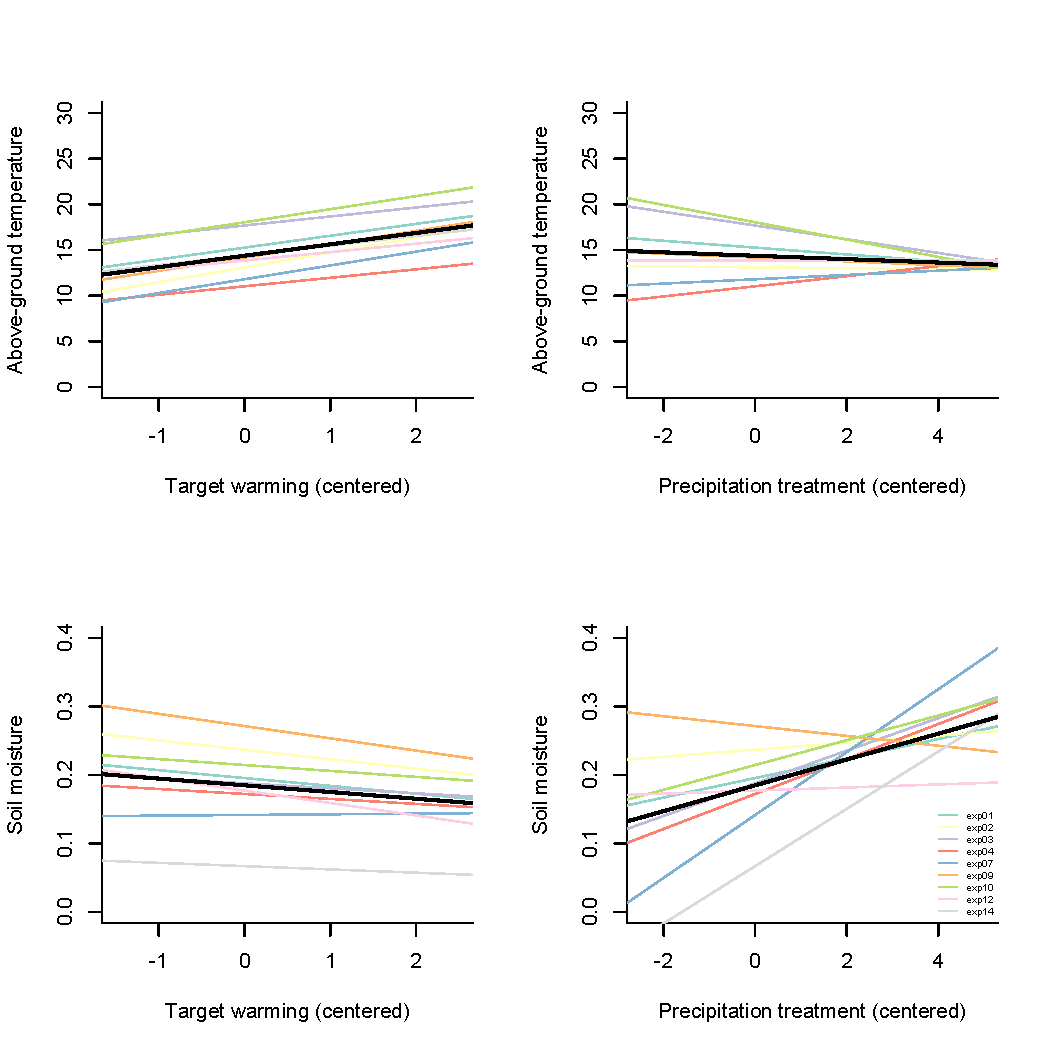
\includegraphics{../../Analyses/soilmoisture/figures/smtempvstargtemppreciptreat_lineslmerALL.pdf}
%  \caption{\textbf{Locations of experiments included in the meta-analysis.}} 
%  \label{fig:soilmois}
%  \end{figure}

% \clearpage
%  \begin{figure}[h]
% \centering
%  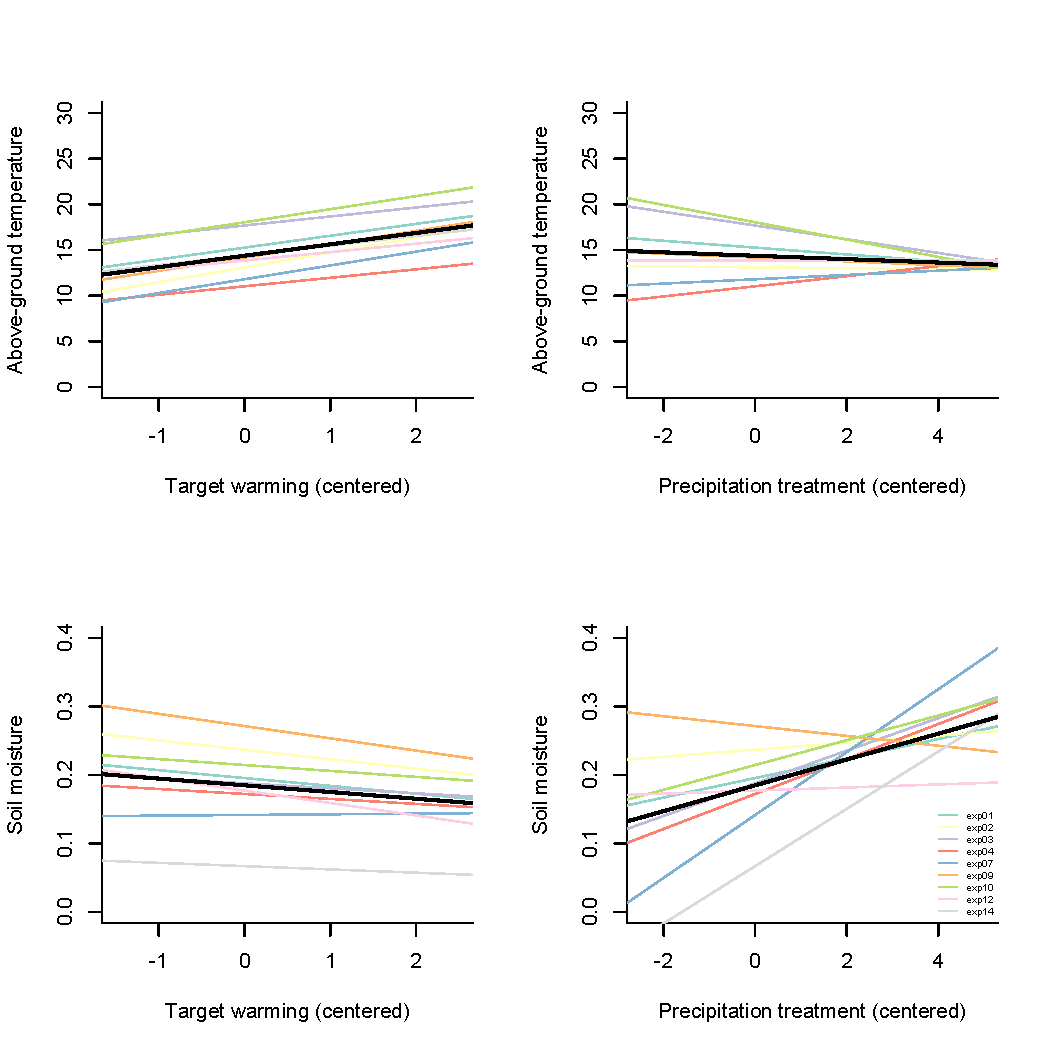
\includegraphics{../../Analyses/soilmoisture/figures/smtempvstargtemppreciptreat_lineslmerALL.pdf}
%  \caption{\textbf{Effects of target temperature and precipitation treatments on soil moisture.}} 
%  \label{fig:soilmois}
%  \end{figure}
% 

% \begin{figure}[h]
% \centering
%  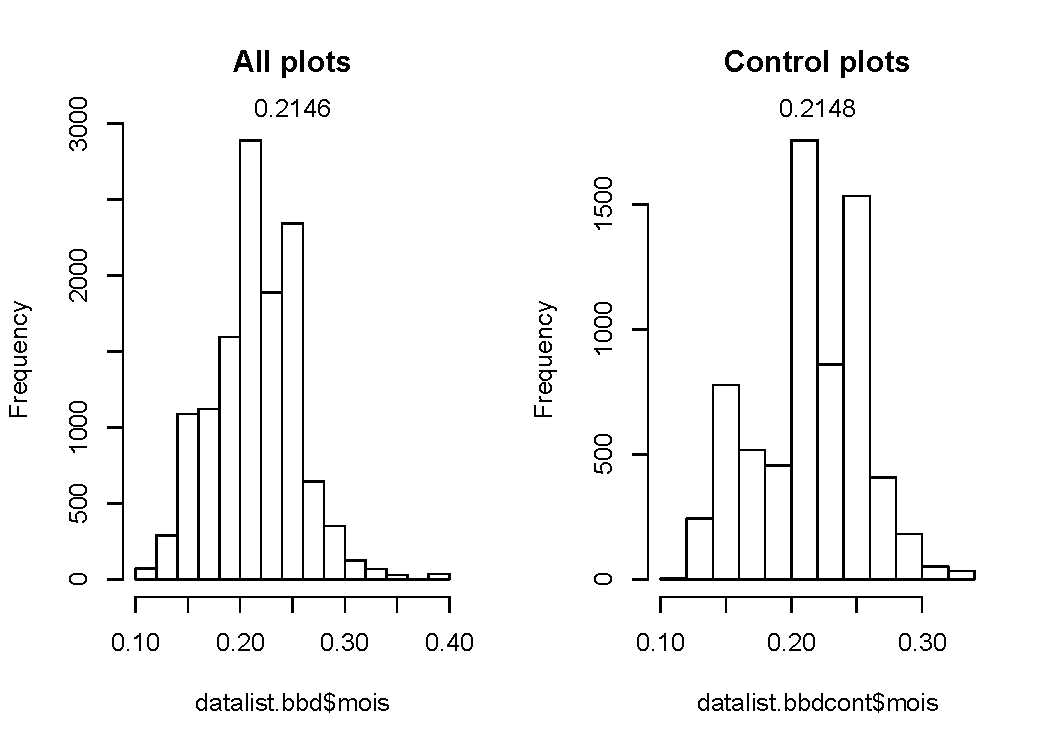
\includegraphics{../../Analyses/soilmoisture/figures/soilmoishist_mn.pdf}
%  \caption{\textbf{Observed daily soil moisture in all plots verus control plots.}} 
%  \label{fig:sm}
%  \end{figure}
% 
% \begin{figure}[h]
% \centering
%  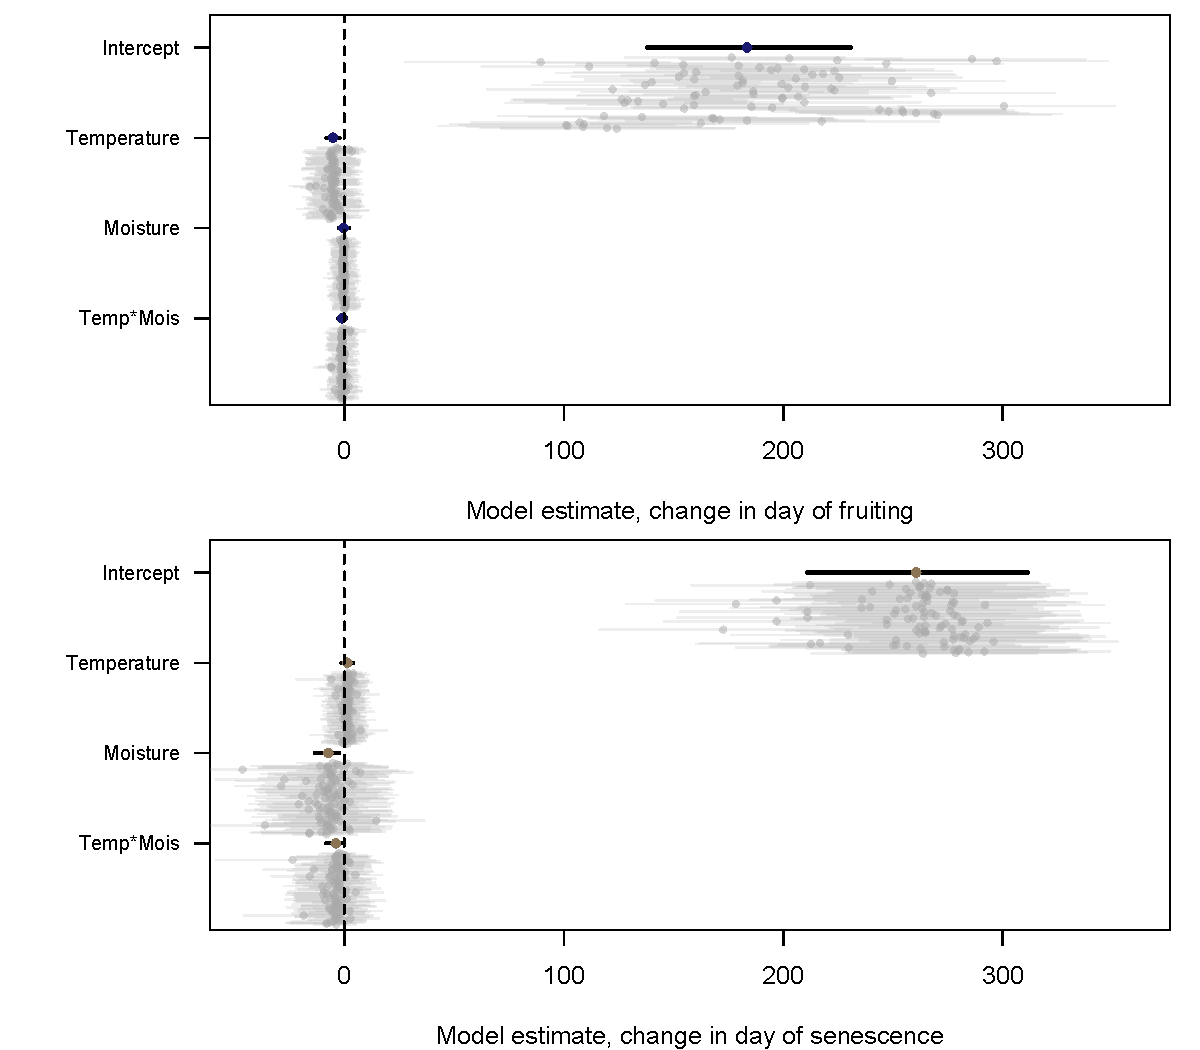
\includegraphics{../../Analyses/soilmoisture/figures/m5bffrdsen.pdf}
%  \caption{\textbf{Model coefficients from fruiting and senescence models (with centered predictors).}} 
%  \label{fig:ff}
%  \end{figure}
 
 \begin{figure}[h]
\centering
 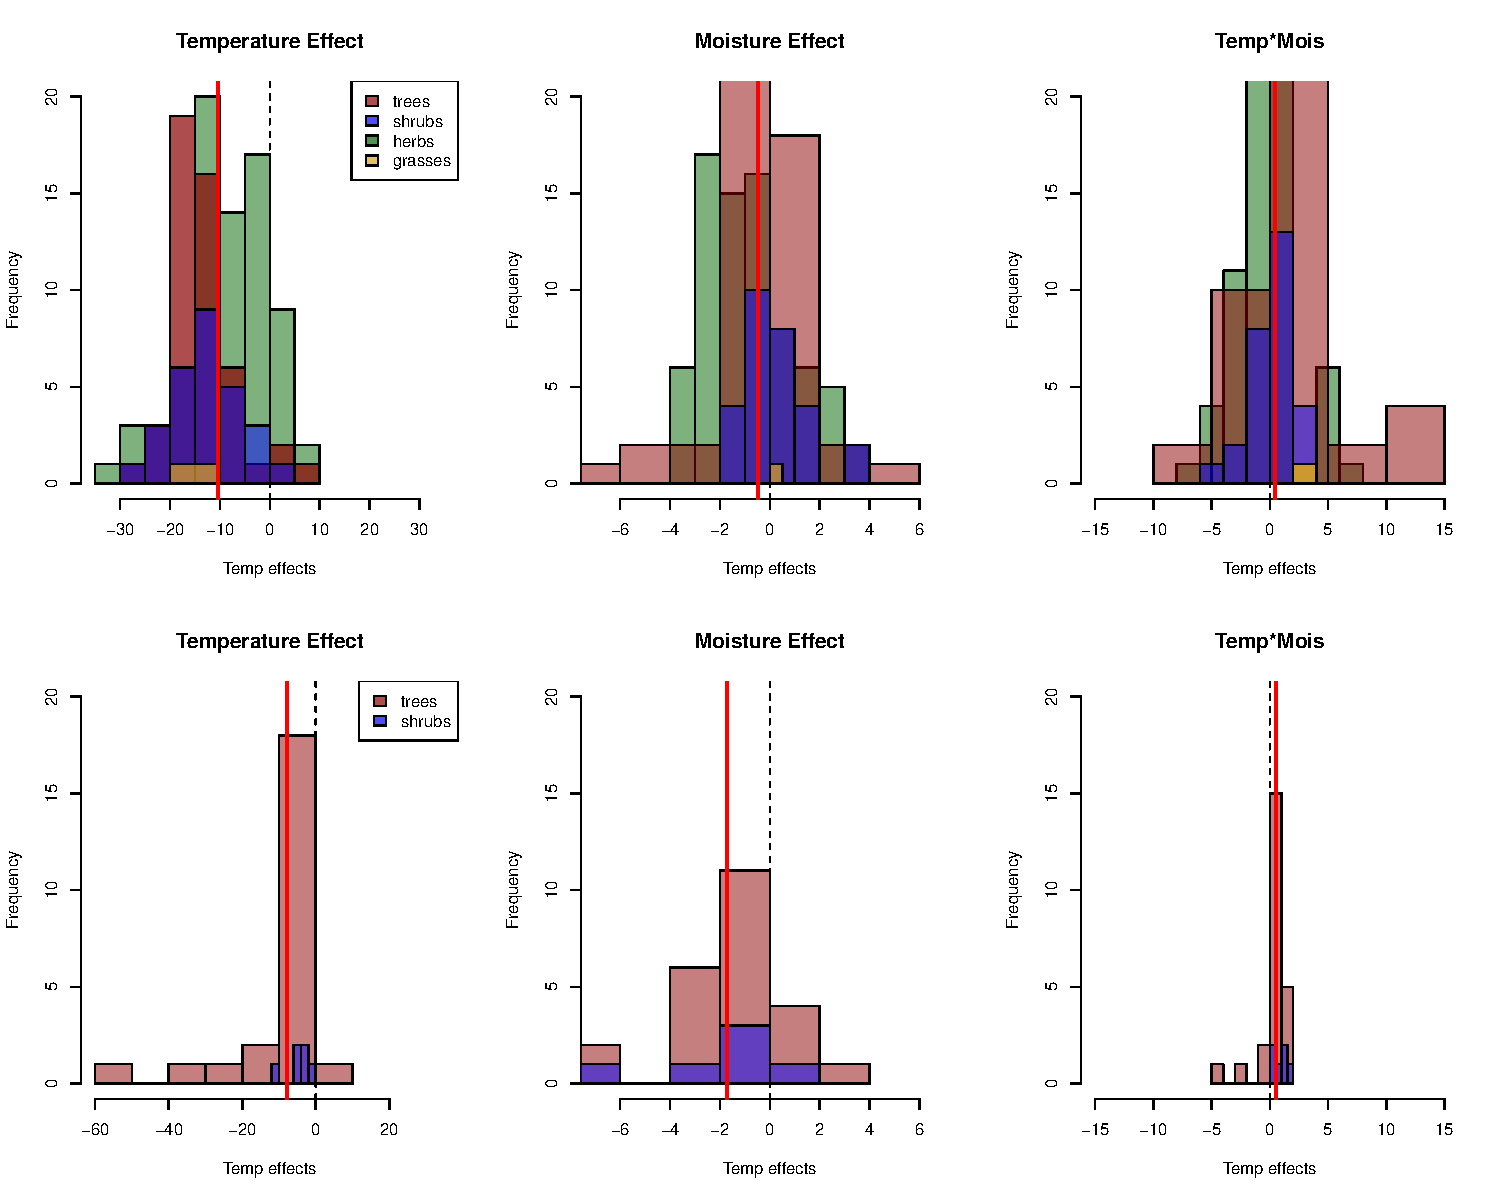
\includegraphics{../../Analyses/soilmoisture/figures/histbbloform_spef.pdf}
 \caption{\textbf{Effects of temperature, soil moisture, and their interaction do not differ strongly across life forms} for leafout (top) and budburst (bottom) models. Histograms show species-level estimated effects for temeprature, soil, and their inteactions across four life forms (trees, shrubs, forms, and grasses).}
 \label{fig:forms}
 \end{figure}

 \begin{figure}[h]
\centering
 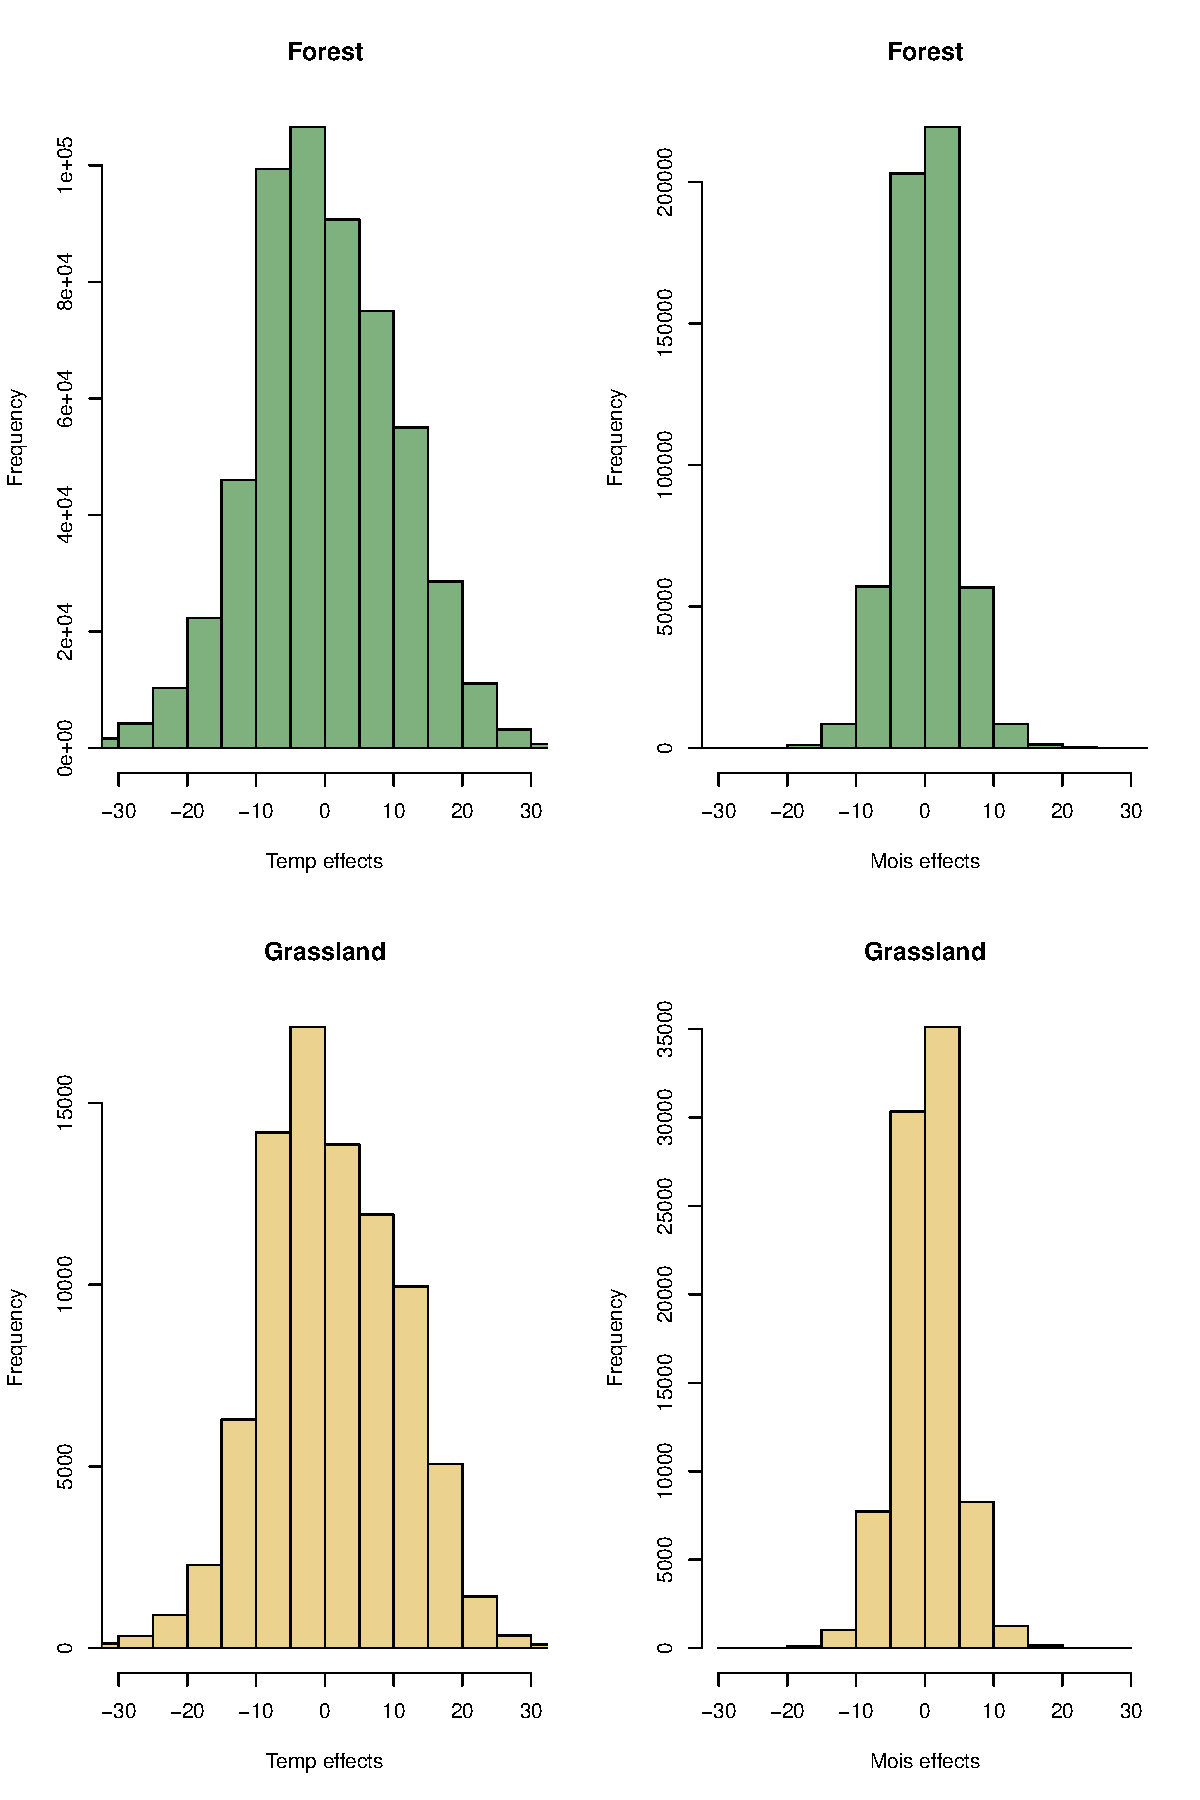
\includegraphics{../../Analyses/soilmoisture/figures/histloecos.pdf}
 \caption{\textbf{Effects of temperature and soil moisture do not differ strongly across ecosystems (forest vs grassland) for leafout (top) and budburst (bottom) models.}.}
 \label{fig:forms}
 \end{figure}
 
 Questions for co-authors:
 \begin{enumerate}
 \item Life forms vs ecosystems figures: Life forms plots histograms of speces level effects whereas ecosystems plots all posterioes- what's your preference?
 \item what do you think of density plots: is it fair to say that variance is greater for tempreature, even though the variances relevative to the mean is about the same?
 \end{enumerate}
%%%%%%%%%%%%%%%%%%%%%%%%%%%%%%%%%%%%%%%%
\end{document}
%%%%%%%%%%%%%%%%%%%%%%%%%%%%%%%%%%%%%%%%
